% -*- mode: latex; -*- mustache tags:  
\documentclass[10pt,twoside,english]{_support/latex/sbabook/sbabook}
\let\wholebook=\relax

\usepackage{import}
\subimport{_support/latex/}{common.tex}

%=================================================================
% Debug packages for page layout and overfull lines
% Remove the showtrims document option before printing
\ifshowtrims
  \usepackage{showframe}
  \usepackage[color=magenta,width=5mm]{_support/latex/overcolored}
\fi


% =================================================================
\title{Learning Object-Oriented Programming, Design and TDD with Pharo}
\author{Stéphane Ducasse}
\series{The Pharo TextBook Collection}

\hypersetup{
  pdftitle = {Learning Object-Oriented Programming, Design and TDD with Pharo},
  pdfauthor = {Stéphane Ducasse},
  pdfkeywords = {Introduction, programming, design, testing, Pharo, Smalltalk}
}


% =================================================================
\begin{document}

% Title page and colophon on verso
\maketitle
\pagestyle{titlingpage}
\thispagestyle{titlingpage} % \pagestyle does not work on the first one…

\cleartoverso
{\small

  Copyright 2017 by Stéphane Ducasse.

  The contents of this book are protected under the Creative Commons
  Attribution-ShareAlike 3.0 Unported license.

  You are \textbf{free}:
  \begin{itemize}
  \item to \textbf{Share}: to copy, distribute and transmit the work,
  \item to \textbf{Remix}: to adapt the work,
  \end{itemize}

  Under the following conditions:
  \begin{description}
  \item[Attribution.] You must attribute the work in the manner specified by the
    author or licensor (but not in any way that suggests that they endorse you
    or your use of the work).
  \item[Share Alike.] If you alter, transform, or build upon this work, you may
    distribute the resulting work only under the same, similar or a compatible
    license.
  \end{description}

  For any reuse or distribution, you must make clear to others the
  license terms of this work. The best way to do this is with a link to
  this web page: \\
  \url{http://creativecommons.org/licenses/by-sa/3.0/}

  Any of the above conditions can be waived if you get permission from
  the copyright holder. Nothing in this license impairs or restricts the
  author's moral rights.

  \begin{center}
    
\includegraphics[width=0.2\textwidth]{_support/latex/sbabook/CreativeCommons-BY-SA.pdf}
  \end{center}

  Your fair dealing and other rights are in no way affected by the
  above. This is a human-readable summary of the Legal Code (the full
  license): \\
  \url{http://creativecommons.org/licenses/by-sa/3.0/legalcode}

  \vfill

  % Publication info would go here (publisher, ISBN, cover design…)
  Layout and typography based on the \textcode{sbabook} \LaTeX{} class by Damien
  Pollet.
}


\frontmatter
\pagestyle{plain}

\tableofcontents*
\clearpage\listoffigures

\mainmatter

\chapter{Revisiting the Die DSL: a Case for Double Dispatch}\label{ch:doubleDispatch}
In Chapter \ref{cha:dsl}, using the Die DSL we could only sum die handles together as in \textcode{2 D20 + 1 D4}. In this new chapter we extend the Die DSL implementation to support the sum of a die with another one or with a die handle (and vice versa). 

One of the challenges is that the message \textcode{+} should be able to manage different types of receivers and arguments. The message will have either a die or a die handle as receiver and arguments, so we should manage the following possibilities: die + die handle, die + die, die handle + die handle, and die handle + die. While this extension at first may look trivial, we will take it as a way to explore double dispatch. 

Double dispatch is a technic that avoids hardcoding type checks and also is able to define incrementally the behavior handling all the possible cases. Indeed double dispatch does not use any explicit conditionals and is the basis of more advanced Design Patterns such as the Visitor. 

Double dispatch is based on the \textit{Don't ask, tell} object-oriented principle applied twice. In the case of the \textcode{+} message, there is a first dispatch to select the adequate method. Then a second dispatch happens when in this method a new message is sent the \textit{argument} of the \textcode{+} message telling this argument the way the current receiver should be summed. This description is clearly too abstract so we will go over a full example to explain it. 
\section{A little reminder}
In a previous chapter you implemented a small DSL to add dice and manage die handles. With this DSL, you could create dice and add them to a die handle. Later on you could sum two different die handles and obtain a new one following the \symbol{34}Dungeons and Dragons\symbol{34} ruling book. 

The following tests show these two behavior: First the dice handle creation and second the sum of die handles.

\begin{displaycode}{plain}
DieHandleTest >> testCreationAdding
	| handle |
	handle := DieHandle new
		addDice: (Dice faces: 6);
		addDice: (Dice faces: 10);
		yourself.
	self assert: handle diceNumber = 2
\end{displaycode}

\begin{displaycode}{plain}
DieHandleTest >> testSummingWithNiceAPI
	| handle |
	handle := 2 D20 + 3 D10.
	self assert: handle diceNumber = 5
\end{displaycode}

The implementation of \textcode{+} was simple since we could only sum die handles together. The method \textcode{+} creates a new handle, adds the dice of the receiver and of the argument to the newly created handle and returns it. 

\begin{displaycode}{plain}
DieHandle >> + aDieHandle
	"Returns a new handle that represents the addition of the receiver and the argument."
	| handle |
	handle := self class new.
	self dice do: [ :each | handle addDie: each ].
	aDieHandle dice do: [ :each | handle addDie: each ].
	^ handle
\end{displaycode}
\section{New requirements }
The first requirement we have is that we want to be able to add two dices together and of course we should obtain a die handle as illustrated by the following test. 

We want to add two dices together:

\begin{displaycode}{plain}
(Die withFaces: 6) + (Die withFaces: 6)
\end{displaycode}

The second requirement is that we want to be able to mix and add a die to a die handle or vice versa as illustrated below: 

\begin{displaycode}{plain}
2 D20 + (Die withFaces: 6)
\end{displaycode}

\begin{displaycode}{plain}
 (Die withFaces: 6) + 2 D20
\end{displaycode}
\section{Turning requirements as tests}
Since we are test-infested, we turn such expected behavior into automatically testable expected behavior: we write them as tests. 

We want to add two dices together:

\begin{displaycode}{plain}
DieTest >> testAddTwoDice
	| hd |
	hd := (Die withFaces: 6) + (Die withFaces: 6).
	self assert: hd dice size = 2.
\end{displaycode}

The second requirement is that we want to be able to mix and add a die to a die handle or vice versa as illustrated by the two following tests: 

\begin{displaycode}{plain}
DieTest >> testAddingADieAndHandle
	| hd |
	hd := (Die faces: 6)
		+
		(DieHandle new
			addDie: 6;
			yourself).
	self assert: hd dice size equals: 2
\end{displaycode}

\begin{displaycode}{plain}
DieHandleTest >> testAddingAnHandleWithADie
	| handle res |
	handle := DieHandle new
		addDie: (Die faces: 6);
		addDie: (Die faces: 10);
		yourself.
	res := handle + (Die faces: 20).
	self assert: res diceNumber equals: 3
\end{displaycode}

Now we are ready to implement such requirements. 
\section{A first implementation}
A first solution is to explicitly type check the argument to decide what to do. 

\begin{displaycode}{plain}
DieHandle >> + aDieOrADieHandle

	^ (aDieOrADieHandle class = DieHandle) 
		ifTrue: [ | handle |
					handle := self class new.
					self dice do: [ :each | handle addDie: each ].
					aDieOrADieHandle dice do: [ :each | handle addDie: each ].
					handle ]
		ifFalse: [ | handle |
					handle := self class new.
					self dice do: [ :each | handle addDie: each ].
					handle addDie: aDie.
					handle  ]
\end{displaycode}

\begin{displaycode}{plain}
Die >> + aDieOrADieHandle
	| selfAsDieHandle |
	selfAsDieHandle := DieHandle new addDie: self.
	^ selfAsDieHandle + aDieOrADieHandle
\end{displaycode}

The problem of this solution is that it does not scale. As soon as we will have other kinds of arguments we will have to check more and more cases. You may think that this is just a spurious argument. But when you have a model that has around 35 different kinds of nodes as in Pillar the document processing system used to produce this book, this kind of testing logic becomes a nightmare to maintain and extend.
\section{Sketching double dispatch}
We can do better.  The logic of the solution we have in mind is quite simple but it may be destabilizing at first.
Let us sketch it.

\begin{itemize}
\item When we execute a method we know its receiver and the kind of receiver we have: it can be a die or a die handle. The method dispatch will select the correct method at runtime. Imagine that we have two \textcode{+} methods for each class \textcode{Die} and \textcode{DieHandle}. When a given method \textcode{+} will be executed, we will know the exact kind of  the receiver. For example, when the method \textcode{+} defined on the class \textcode{Die} will be executed, we will know that the receiver is a die (instance of this class). Similarly when the method \textcode{+} defined on the class \textcode{DieHandle} will be executed, we will know that the message receiver is a die handle. This is the power of method dispatch: it selects the right method based on the message receiver.
\end{itemize}

\begin{itemize}
\item Then the idea is to tell the argument that we want to sum it with that given receiver. It means that each \textcode{+} method on the different class has just to send a different message based on the fact that the receiver was a die or a die handle to its argument and let the method dispatch to act once again. After this second dispatch, the correct method will be selected. 
\end{itemize}

But let us makes this really concrete.
\section{Adding two dice}
Let us step back and start by supporting the sum of two dice. This is rather simple we create and return a die 
handle to which we add the receiver and the argument.

\begin{displaycode}{plain}
Die >> + aDie
	
	^ DieHandle new 
		addDie: self; 
		addDie: aDie; yourself
\end{displaycode}

Our first test should pass \textcode{testAddTwoDice}.
But this solution does not support the fact that the argument can be either a die or a die handle.
\section{Adding a die and a die or a handle}
Now we want to handle the fact that we can add a die or a die handle to the receiver as illustrated by the test \textcode{testAddingADieAndHandle}.

\begin{displaycode}{plain}
DieTest >> testAddingADieAndHandle
	| hd |
	hd := (Die faces: 6)
		+
		(DieHandle new
			addDie: 6;
			yourself).
	self assert: hd dice size equals: 2
\end{displaycode}

The previous method \textcode{+} is definitively what we want to do when we have two dice. So let us rename it as \textcode{sumWithDie:} so that we can invoke it later. 

\begin{displaycode}{plain}
Die >> sumWithDie: aDie

	^ DieHandle new
		addDie: self;
		addDie: aDie; yourself
\end{displaycode}

Now what we can do is to implement \textcode{+} as follows. Notice that we named the argument \textcode{aDicable} because we want to convey that the argument can be either a die or a die handle. 

\begin{displaycode}{plain}
Die >> + aDicable	
	^ aDicable sumWithDie: self
\end{displaycode}

We tell the argument \textcode{aDicable} (which can be a die or a die handle) that we want to sum to it a die (we know that  \textcode{self} in this method is a \textcode{Die} because this is the method of this class that is executed). When rewritting the \textcode{+} method, we switched \textcode{self} and \textcode{aDicable} to send the new message \textcode{sumWithDie:} to the argument (\textcode{aDicable}). This switch kicks a new method dispatch and we finally have a double dispatch (one of \textcode{+} and one for \textcode{sumWithDie:}).

In our two tests \textcode{testAddTwoDice} and \textcode{testAddingADieAndHandle} we know that the receiver is a die because the method is defined in the class of \textcode{Die}. At this point the test \textcode{testAddTwoDice} should pass because we are adding two dice as shown in Figure \ref{figDieDoubleDispatchPartialArgDie}.


\begin{figure}

\begin{center}
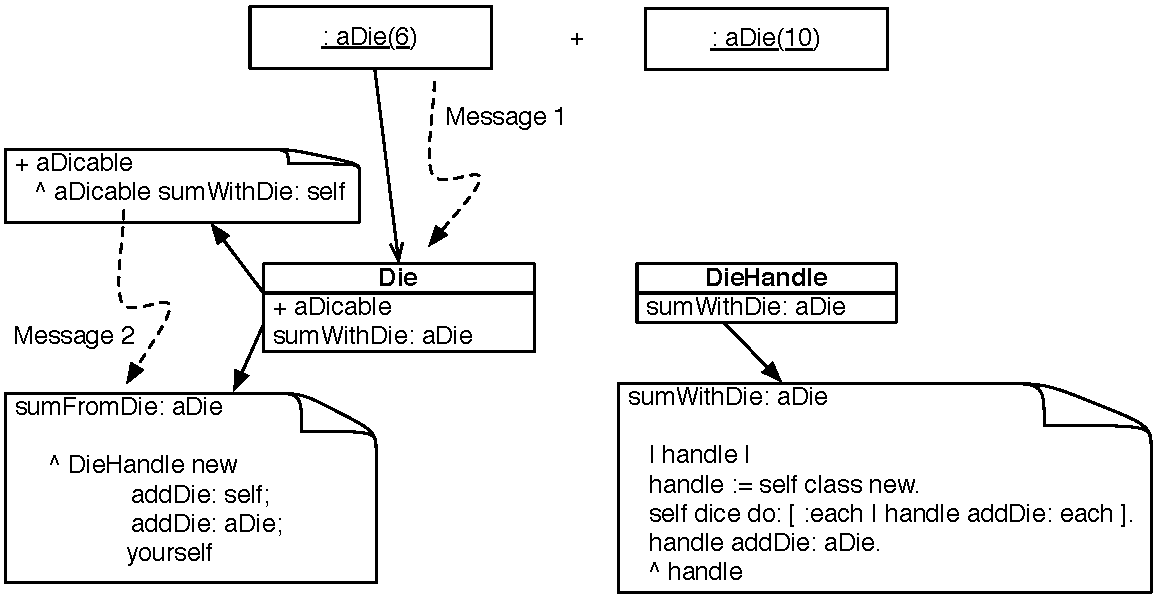
\includegraphics[width=0.7\textwidth]{/Users/ducasse/Workspace/FirstCircle/MyBooks/Bk-Writing/PharoBooks/LearningOOPWithPharoTrans/_result/pdf/Chapters/DoubleDispatch/figures/DieDoubleDispatchPartialArgDie.pdf}\caption{Summing two dice and be prepared for more.\label{figDieDoubleDispatchPartialArgDie}}\end{center}
\end{figure}

\section{When the argument is a die handle}
Now we still have to find a solution for the case where the argument to the message \textcode{+} is a die handle.
In fact, the argument will receive the message \textcode{sumWithDie:}. Therefore if we define a method with that name in the class \textcode{DieHandle} it will be executed when the argument of message \textcode{+} is a die handle.

We know how to sum a die with a die handle: we simply create a new die handle, add all the die of the previous die handle to the new one and add the argument too. 

So we just have to define the method \textcode{sumWithDie:} to the class \textcode{DieHandle} implementing this logic. 

\begin{displaycode}{plain}
DieHandle >> sumWithDie: aDie
	| handle |
	handle := self class new.
	self dice do: [ :each | handle addDie: each ].
	handle addDie: aDie.
	^ handle
\end{displaycode}

Now we are able to sum a die with a die handle as shown in Figure \ref{figDieDoubleDispatchPartialArgDieHandle}. The test \textcode{testAddingADieAndHandle} should now pass.


\begin{figure}

\begin{center}
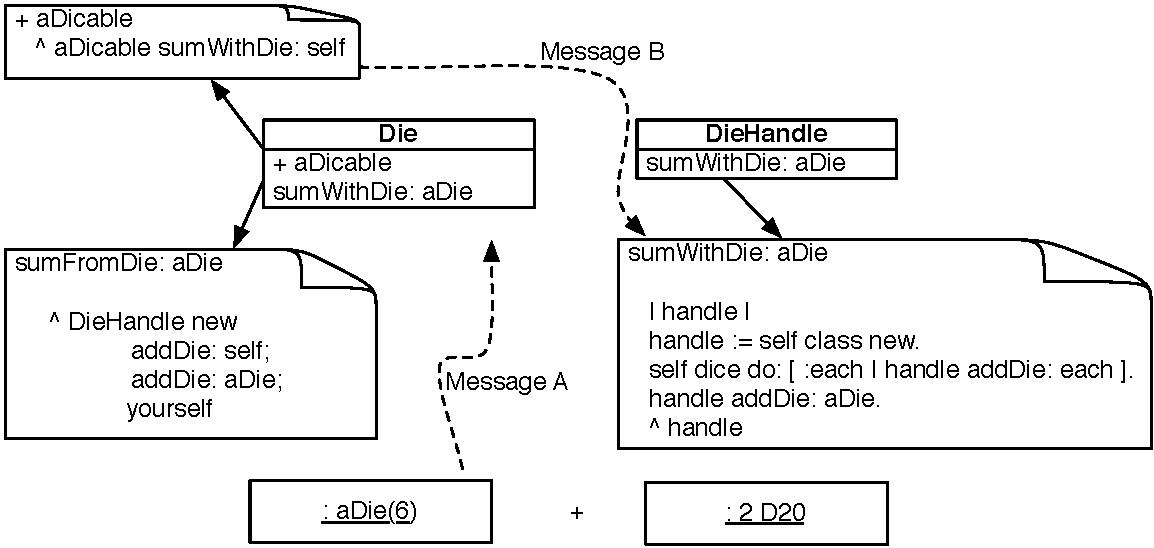
\includegraphics[width=0.9\textwidth]{/Users/ducasse/Workspace/FirstCircle/MyBooks/Bk-Writing/PharoBooks/LearningOOPWithPharoTrans/_result/pdf/Chapters/DoubleDispatch/figures/DieDoubleDispatchPartialArgDieHandle.pdf}\caption{Summing a die and a dicable.\label{figDieDoubleDispatchPartialArgDieHandle}}\end{center}
\end{figure}

\section{Stepping back}
You may ask why this is working. We defined two methods \textcode{sumWithDie:} one on class \textcode{Die} and one on the class \textcode{DieHandle}
and when the method \textcode{+} on class \textcode{Die} will send the message \textcode{sumWithDie:} to either a die or a die handle, the message dispatch will select the correct method \textcode{sumWithDie:} for us as shown in Figure \ref{figDieDoubleDispatchPartial}.


\begin{figure}

\begin{center}
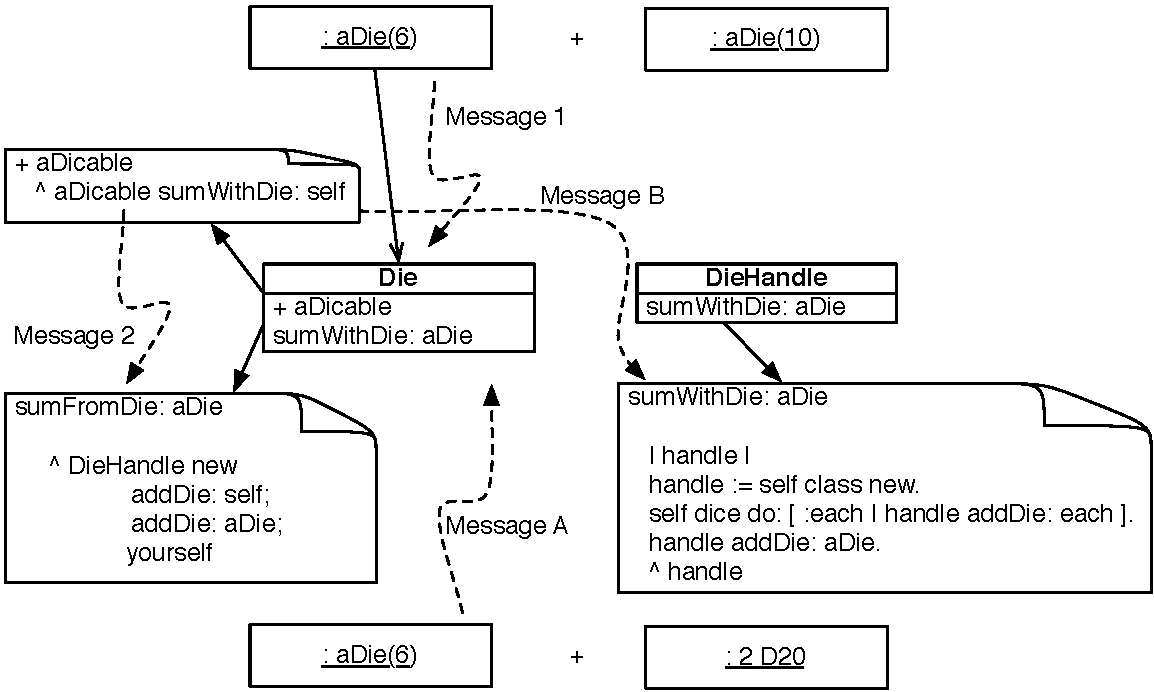
\includegraphics[width=0.9\textwidth]{/Users/ducasse/Workspace/FirstCircle/MyBooks/Bk-Writing/PharoBooks/LearningOOPWithPharoTrans/_result/pdf/Chapters/DoubleDispatch/figures/DieDoubleDispatchPartial.pdf}\caption{Summing a die and a dicable\label{figDieDoubleDispatchPartial}}\end{center}
\end{figure}

\section{Now a DieHandle as receiver}
Our solution does not handle the case where the receiver is a die handle. This is what we will address now. 
Now we are ready to apply the same pattern than before but for the case where the receiver is a die handle. We will just say to the argument of the message \textcode{+} that we want to sum it with a \textit{die handle} this time.

We know how to sum two die handles, it is the code we already defined in the previous chapter. We rename the \textcode{+} method
as \textcode{sumWithHandle:} to be able to invoke it while redefining the method \textcode{+}. Basically this method creates a new handle, then adds the dice of the receiver and the argument to it and returns the new handle.

\begin{displaycode}{plain}
DieHandle >> sumWithHandle: aDieHandle
	| handle |
	handle := self class new.
	self dice do: [ :each | handle addDie: each ].
	aDieHandle dice do: [ :each | handle addDie: each ].
	^ handle
\end{displaycode}

Now we can define a more powerful version of \textcode{+} by simply sending the message \textcode{sumWithHandle:} to the \textbf{argument} (aDicable) of the message \textcode{+}. Again we send a message to the argument (\textcode{aDicable}) to kick in a new message lookup and dispatch  for the message \textcode{sumWithHandle:}.

\begin{displaycode}{plain}
DieHandle >> + aDicable
	^ aDicable sumWithHandle: self
\end{displaycode}

We said that this is version of \textcode{+} is more powerful than the one of \textcode{sumWithHandle:} because once we will implement the missing method \textcode{sumWithHandle:} on the class \textcode{Die}, the \textcode{+} method will be able to sum die handle with die or die handle. 


\begin{figure}

\begin{center}
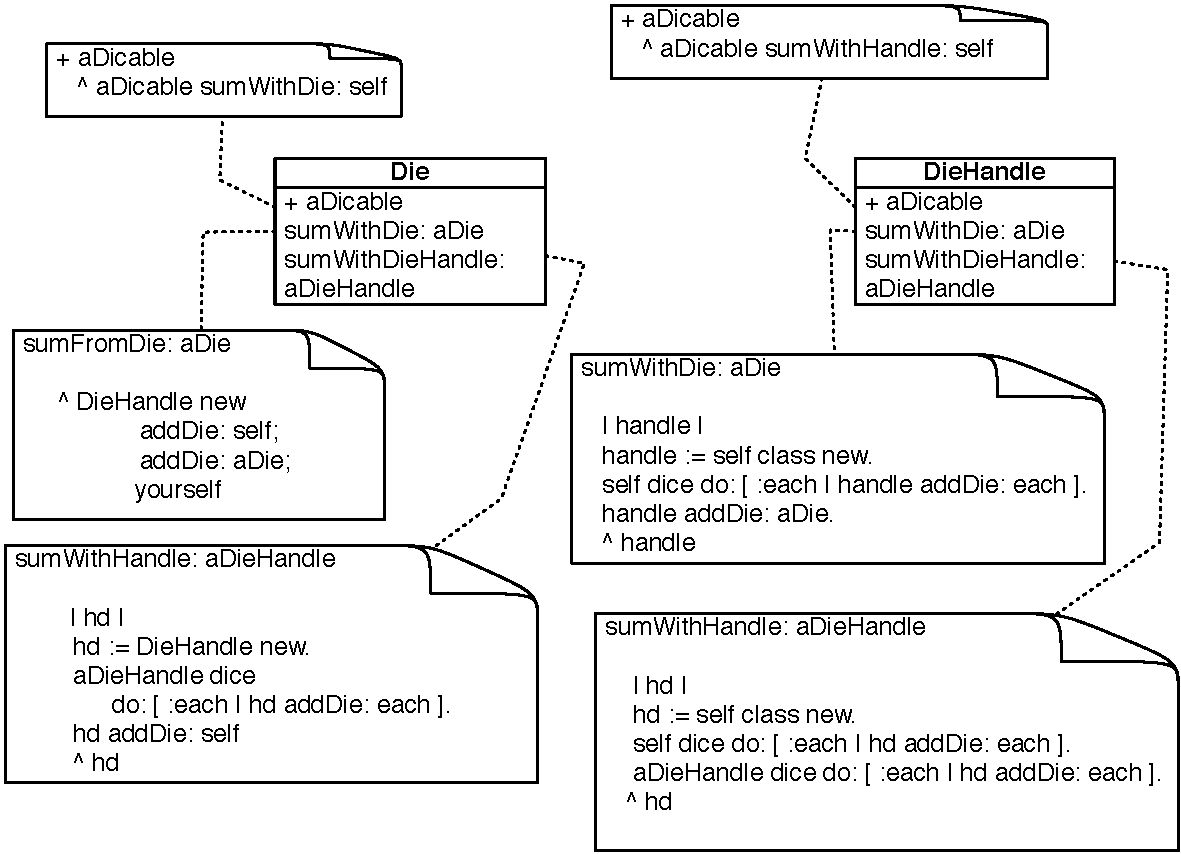
\includegraphics[width=0.9\textwidth]{/Users/ducasse/Workspace/FirstCircle/MyBooks/Bk-Writing/PharoBooks/LearningOOPWithPharoTrans/_result/pdf/Chapters/DoubleDispatch/figures/DieDoubleDispatchFull.pdf}\caption{Handling all the cases: summing a die/die handle with a die/die handle .\label{figDieDoubleDispatchFull}}\end{center}
\end{figure}


Up until here we did not change much and all the tests adding two die handle should continue to run. 
\section{sumWithHandle: on Die class}
To get the possibility to sum a die handle with a single die, we just have to define a new method \textcode{sumWithHandle:} on the \textcode{Die} class. 
The logic is similar to the one adding one die to one die handle

\begin{displaycode}{plain}
Die >> sumWithHandle: aDieHandle
	| handle |
	handle := DieHandle new.
	aDieHandle dice do: [ :each | handle addDie: each ].
	handle addDie: self
	^ handle
\end{displaycode}

Note that we could have  sent the message \textcode{aDieHandle sumWithDie: self} as body of \textcode{sumWithHandle:} definition.

Figure \ref{figDieDoubleDispatchFull} shows the full set up. We suggest to follow the execution of messages for the different cases to understand that just sending a new message to the argument and relying on method dispatch produces modular conditional execution.
Now the following test should pass and we are done.

\begin{displaycode}{plain}
DieHandleTest >> testAddingAnHandleWithADie
	| handle res |
	handle := DieHandle new
		addDie: (Die faces: 6);
		addDie: (Die faces: 10);
		yourself.
	res := handle + (Die faces: 20).
	self assert: res diceNumber equals: 3
\end{displaycode}
\section{Conclusion}
When we step back, we see that we applied twice the \textit{Don't ask, tell} principle:
First the message \textcode{+} selects the corresponding methods in either \textcode{Die} or \textcode{DieHandle} classes. Then a more specific message is sent to the argument and the dispatch kicks in again selecting the correct method for the messages \textcode{sumWithDie:} or \textcode{sumWithHandle:}.

In this chapter we presented double dispatch. The idea is to use method dispatch two times.
While the resulting design is simple, it is not trivial to deeply understand and it requires time to digest double dispatch. 
At its core, double dispatch relies on the fact that sending a message to an object selects the correct method -- and 
sending another message to the message argument will select a new method. Therefore we have effectively selected a method according to the receiver and the argument of a message.

Double dispatch is the basis for the Visitor Design pattern that is effective when dealing with complex data structure such as documents, compilers. In such context it is not rare to have more than 30 or 40 different nodes that should be manipulated together to produce specific behavior. 


% lulu requires an empty page at the end. That's why I'm using
% \backmatter here.
\backmatter

% Index would go here
\bibliographystyle{abbrv}
\bibliography{others.bib}
\end{document}
